\chapter{Polynomial Multiplication}
\begin{algoprob}
	\problemtitle{{Polynomial Multiplication}}
	\probleminput{Given 2 univariate polynomials of degree $n-1$ by 2 arrays of their coefficients $(a_0,\dots, a_{n-1})$ and $(b_0,\dots, b_{n-1})$ such that $A(x)=a_0+a_1x+\cdots+ a_{n-1}x^{n-1}$ and $B(x)=b_0+b_1x+\cdots+b_{n-1}x^{n-1}$ respectively}
	\problemquestion{Given 2 polynomials of degree $n-1$ find their product polynomial $C(x)=A(x)B(x)$ of degree $2n-2$ by returning the array of their coefficients.}
\end{algoprob}
\section{Naive Algorithm}
We can do this naively by calculating each coefficient of $C$ in $O(n)$ time since for any $i\in\{0,\dots, 2n-2\}$ $$c_i=\sum_{j=0}^ia_jb_{i-j}$$Since there are $2n-1=O(n)$ total coefficient of $C$ it takes total $O(n^2)$ time. In the following section we will do this in $O(n\log n)$ time.
\section{Strassen-Sch\"{o}nhage Algorithm}
Before diving into the algorithm first let's consider how many ways we can represent a polynomial. Often changing the representation helps solving the problem in less time.\begin{itemize}
	\item \textbf{Coefficients}: We can represent a polynomial by giving the array of all its coefficient.
	\item \textbf{Point-Value Pairs}: We can evaluate the polynomial in distinct $n$ points and give all the point-value pairs. This also uniquely represents a polynomial since there is exactly one polynomial of degree $n-1$ which passes through all these points. 
\end{itemize}
\begin{Theorem}{}{}
	Given $n$ distinct points $(x_0,y_0),\dots, (x_{n-1},y_{n-1})$ in $\bbR^2$ there is an unique $(n-1)-$degree polynomial $P(x)$ such that $P(x_i)=y_i$ for all $i\in \llbracket n-1\rrbracket$
\end{Theorem}
\parinn

Since we want to find the polynomial $C(x)=A(x)B(x)$ and $C(x)$ has degree $2n-2$, we will evaluate the polynomials $A(x)$ and $B(x)$ in $2n-1$ distinct points. So we will have the algorithm like this:
%\begin{figure}[h]
%	\centering
%	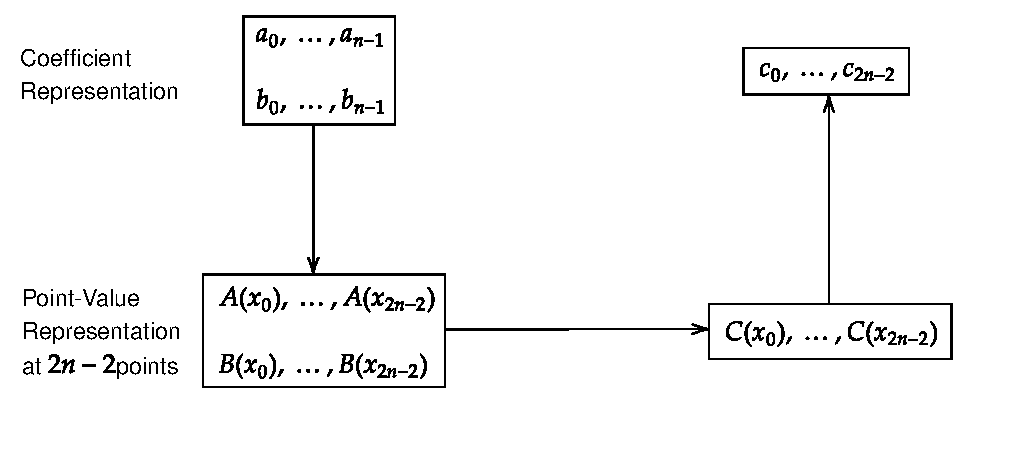
\includegraphics{images/poly-mult}
%\end{figure}
\begin{center}

\begin{tikzpicture}[node distance=3cm, thick]
	
	% Define the rectangles
	\node[draw, rectangle, minimum width=3cm, minimum height=1.5cm] (rect1) at (0, 1.5) {$ \begin{array}{l}
			a_{0} ,\dotsc ,a_{n-1}\\
			\\
			b_{0} ,\dotsc ,b_{n-1}
		\end{array}$};
	\node[draw, rectangle, minimum width=3cm, minimum height=1.5cm] at (0,-3) (rect2) {$ \begin{array}{l}
			A( x_{0}) ,\dotsc ,A( x_{2n-2})\\
			\\
			B( x_{0}) ,\dotsc ,B( x_{2n-2})
		\end{array}$};
	\node[draw, rectangle, minimum width=3cm, minimum height=1cm]  at (8, 1.5) (rect3) {$c_{0} ,\dotsc ,c_{2n-2}$};
	\node[draw, rectangle, minimum width=4cm, minimum height=1.5cm] at (8,-3) (rect4) {$C( x_{0}) ,\dotsc ,C( x_{2n-2})$};
	% Define the text blocks on the left
	\node[align=left] (text1) at (-4, 1.5) {Coefficient\\ Representation};
	\node[align=left] (text2) at (-4, -3) {Point-Value\\ Representation\\ at $\displaystyle 2n-2$ points};
	
	% Draw dotted helper lines (optional for alignment visualization)
	\draw[-Stealth] (rect1.south) -- (rect2.north);
	\draw[-Stealth] (rect2.east) -- (rect4.west);
	\draw[-Stealth] (rect4.north) -- (rect3.south);	
\end{tikzpicture}
\end{center}
\subsection{Finding Evaluations of Multiplied Polynomial}

Suppose we were given $A(x)$ and $B(x)$ evaluated at $2n-1$ distinct points $x_0,\dots, x_{2n-2}$. Then we can get $C(x)$ evaluated at $x_0,\dots, x_{2n-2}$ by $$C(x_i)=A(x_i)B(x_i)\ \forall\ i\in \llbracket 2n-2\rrbracket$$Since there are $O(n)$ many points and for each point it takes constant time to multiply we can find evaluations of $C$ at $x_0,\dots, x_{2n-2}$ in $ O(n)$ time.
\subsection{Evaluation of a Polynomial at Points}\label{fft}
\begin{question}{}{}
	Suppose there is only one point, $x_0$. Can we evaluate a $n-1$ degree polynomial $A(x)=\sum\limits_{i=0}^{n-1}a_ix^i$ at $x_0$ efficiently?
\end{question}
We can rewrite $A(x)$ as $$A(x)=a_0+x(a_1+x(a_2+x(a_3+\cdots (a_{n-1}+x(a_n))\cdots )))$$In this represent it is clear that we have to do $n$ additions and $n$ multiplications to find $A(x_0)$. Hence we can evaluate a $n-1$ degree polynomial at a point in $O(n)$ time


But we have $O(n)$ points. And if each point takes $O(n)$ time to find the evaluation of the polynomial then again it will take total $O(n^2)$ time. We are back to square one. So instead we will evaluate the polynomial in some special points and we will evaluate in all of them in $O(n\log n)$ time. So now the problem we will discuss now is to find some special $n$ points where we can evaluate a $n-1$-degree polynomial in $O(n\log n)$ time.
\parinf

\textbf{Idea:} Evaluate at roots of unity and use Fast Fourier Transform
\parinn

Assume $n$ is a power of 2. NWe have the polynomial $A(x)=\sum\limits_{i=0}^{n-1}a_ix^i$. So now consider the following two polynomials $$A^0(x)=a_0+a_2x+a_4x^2+\cdots+a_{n-2}x^{\frac{n}2-1}\qquad A^1(x)=a_1+a_3x+a_5x^2+\cdots+a_{n-1}x^{\frac{n}2-1}$$Certainly we have $$A(x)=A^0(x^2)+xA^1(x^2)$$Hence we can get $A(1)$ and $A(-1)$ by $$A(1)=A^0(1)+A^1(1)\qquad A(-1)=A^0(1)-A^1(1)$$Hence like this by evaluating two $\frac{n}2-1$ degree polynomials at one point we get evaluation of $A$ at two points. More generally for any $y\geq 0$ we have$$A(\sqrt{y})=A^0(y)+\sqrt{y}A^1(y)\qquad A(-\sqrt{y})=A^0(y)-\sqrt{y}A^1(y)$$So by recursing like this evaluating at $1,-1$ we can get evaluations of $A$ at $n^{th}$ roots of unity.

Let $$\om_n^k=n^{th}\text{ root of unity for }k\in\llbracket n-1\rrbracket = e^{i\frac{k}{n}2\pi}=\cos\lt(\frac{k}{n}2\pi\rt)+i\sin s\lt(\frac{k}{n}2\pi\rt)$$Hence we have \begin{align*}
	A\lt(\om_n^k\rt)&=A^0\lt(\om_n^{2k}\rt)+\om_n^kA^1\lt(\om_n^{2k}\rt)=A^0\lt(\om_{\frac{n}2}^{k}\rt)+\om_n^kA^1\lt(\om_{\frac{n}2}^{k}\rt)\\
	A\lt(-\om_n^k\rt)=A\lt(\om_n^{\frac{n}2+k}\rt)&=A^0\lt(\om_n^{2k}\rt)-\om_n^kA^1\lt(\om_n^{2k}\rt)=A^0\lt(\om_{\frac{n}2}^{k}\rt)-\om_n^kA^1\lt(\om_{\frac{n}2}^{k}\rt)
\end{align*}Hence now we will solve the following problem:
\begin{algoprob}
	\problemtitle{Recursive-DFT}
	\probleminput{$(a_0,\dots, a_{n-1})$ representing $(n-1)-$degree polynomial $A(x)=\sum\limits_{i=0}^{n-1}a_ix^i$}
	\problemquestion{Find the evaluations of the polynomial $A(x)$ in all $n^{th}$ roots of unity}
\end{algoprob}

\vspace*{5mm}\parinf
Since $A^0$ and $A^1$ have degree $\frac{n}2-1$ we can use recursion. Hence the algorithm is 
\begin{algorithm}\SetKwComment{Comment}{// }{}
	\DontPrintSemicolon
	\KwIn{$A=(a_0,\dots, a_{n-1})$ such that $A(x)=a_0+a_1x+\cdots+ a_{n-1}x^{n-1}$}
	\KwOut{$A(x)$ evaluated at $n^{th}$ roots of unity $\om_n^k$ for all $k\in\llbracket n-1\rrbracket$}
	\Begin{
	\If{$n==1$}{\Return{$A[0]$}}
	$A^0\longleftarrow (A[0],A[2],\dots,A[n-2])$\;	
	$A^1\longleftarrow(A[1],A[3],\dots,A[n-1])$\;
	$Y^0\longleftarrow 	\prb{Recursive-DFT}(A^0)$\;
	$Y^1\longleftarrow 	\prb{Recursive-DFT}(A^1)$\;		
	\For{$k=0$ to $\frac{n}{2}-1$}{
		
	$Y[k]\longleftarrow Y^0[k]+\om_n^kY^1[k]$\Comment*{$	A\lt(\om_n^k\rt)=A^0\lt(\om_{\frac{n}2}^{k}\rt)+\om_n^kA^1\lt(\om_{\frac{n}2}^{k}\rt)$}
	$Y\lt[k+\frac{n}{2}\rt]\longleftarrow Y^0[k]-\om_n^{\frac{n}2+k}Y^1[k]$\Comment*{$	A\lt(-\om_n^k\rt)=A^0\lt(\om_{\frac{n}2}^{k}\rt)-\om_n^kA^1\lt(\om_{\frac{n}2}^{k}\rt)$}
}
\Return{Y}
}
		\caption{\prb{Recursive-DFT}$(A)$}
	\end{algorithm}

\textbf{Time Complexity}: $T(n)=2T\lt(\frac{n}2\rt)+O(n)=O(n\log n)$.\parinn

 Therefore we can evaluate a $n-1$ degree polynomial in all the $n^{th}$ roots of unity in $O(n\log n)$ time. Hence with this algorithm we will get evaluations of the polynomial $C(x)=A(x)B(x)$ in all the $2n^{th}$ roots of unity. Now we need to interpolate the polynomial $C(x)$ from its evaluations. We will describe the process in the next subsection.
 \subsection{Interpolation from Evaluations at Roots of Unity}In this section we will show how to interpolate a $n-1$ degree polynomial from evaluations at all $n^{th}$ roots of unity. Previously we had $$\underbrace{\mat{C\lt(\om^0_n\rt)\\ C\lt(\om^1_n\rt)\\ C\lt(\om^2_n\rt)\\ \vdots\\ C\lt(\om^{n-1}_n\rt)}}_{Y}=\underbrace{\mat{1 & \om^0_n & \om ^{0\cdot 2}& \cdots & \om^{0\cdot (n-1)}\\  1 & \om^1_n & \om ^{1\cdot 2}& \cdots & \om^{1\cdot (n-1)}\\ 1 & \om^2_n & \om ^{2\cdot 2}& \cdots & \om^{2\cdot (n-1)}\\ \vdots & \vdots & \vdots & \ddots & \vdots\\ 1 & \om^{n-1}_n & \om ^{(n-1)\cdot 2}& \cdots & \om^{(n-1)\cdot (n-1)}}}_{V=\text{ Vandermonde Matrix}}\underbrace{\mat{c_0\\ c_1\\ c_2\\ \vdots \\ c_{n-1}}}_{C}$$
 
 Now vandermonde matrix is invertible since all the $n^{th}$ roots are distinct. Therefore $C=V^{-1}Y$. But we can not do a matrix inversion to interpolate the polynomial because that will take $O(n^2)$ time. Instead we have this beautiful result:
 \begin{lemma}{}{}
 	$\lt(V^{-1}\rt)_{j,k}=\frac1n\om_n^{-jk}$ for all $0\leq j,k\leq n-1$
 \end{lemma}
\begin{proof}
	Consider the matrix $n\times n$ matrix $T$ such that $(T)_{j,k}=\frac1n\om_n^{-jk}$. Now we will show $VT=I$ This will confirm that $V^{-1}=T$. Now $$\sum_{k=0}^{n-1} (V)_{i,j}\, (T)_{j,k}=\sum_{k=0}^{n-1} \om^{ij}_n\times \frac1n\om_n^{-jk}=\frac1n\sum_{k=0}^{n-1}\lt(\om^{i-k}_n\rt)^j=\begin{cases}
		\dfrac1n\dps{\sum\limits_{k=0}^{n-1}}1=1& \text{when $i=k$}\\[5mm] \dfrac1n \dfrac{1-\om^n_n}{1-\om} =0 & \text{when $i\neq k$}
	\end{cases} $$Hence in $VT$ there are $1'$s on the diagonal and rest of the locations are $0$. Hence $VT=I$. So $V^{-1}=T$.
\end{proof}
Hence we can see the inverse of the vandermonde matrix is also a vandermode matrix with a scaling factor. We will denote $y_i=C\lt(\om_n^{i}\rt)$ for $i\in\llbracket n-1\rrbracket$ since these values are given to us some how and we have to find the corresponding polynomial. Therefore we have $$\underbrace{\mat{c_0\\ c_1\\ c_2\\ \vdots \\ c_{n-1}}}_{C}=\frac1n\underbrace{\mat{1 & 1 & 1& \cdots & 1\\  1 & \om^{-1}_n & \om ^{-1\cdot 2}& \cdots & \om^{-1\cdot (n-1)}\\ 1 & \om^{-2}_n & \om ^{-2\cdot 2}& \cdots & \om^{-2\cdot (n-1)}\\ \vdots & \vdots & \vdots & \ddots & \vdots\\ 1 & \om^{-(n-1)}_n & \om ^{-(n-1)\cdot 2}& \cdots & \om^{-(n-1)\cdot (n-1)}}}_{V^{-1}}\underbrace{\mat{y_0\\ y_1\\ y_2\\ \vdots\\ y_{n-1}}}_{Y}$$
\begin{observation*}
	$nc_j=y_0+y_1\om_n^{-j}+y_2\om_n^{-2j}+\cdots+y_{n-1}\om_n^{-(n-1)j}$ for all $j\in\llbracket n-1\rrbracket$.
\end{observation*}
We can also see this situation as we have the polynomial $Y(x)=y_0+y_1x+y_2x^2+\cdots +y_{n-1}x^{n-1}$ and $c_j$ is just $Y(x)$ evaluated as $\om^{-j}_n=\om_n^{n-j}$ multiplied by $n$. Hence we just reindex the $n^{th}$ roots of unity and evaluate $Y$ $n^{th}$ roots of unity in $O(n\log n)$ time using the algorithm described in \autoref{fft}